\documentclass[12pt]{ctexart}

\usepackage{geometry}
\geometry{a4paper,scale=0.8}
\usepackage{graphicx}
\usepackage{minted}
\usepackage{hyperref}

\setminted{
    fontsize=\small,           % 字体大小
    baselinestretch=1.0,       % 行间距
    linenos=true,              % 行号
    frame=lines,               % 边框样式
    framesep=2mm,              % 边框间距
    rulecolor=\color{black},   % 边框颜色
    numbersep=5pt,             % 行号间距
    breaklines=true,           % 自动换行
    breakanywhere=false,       % 不在任意位置断行
    showspaces=false,          % 不显示空格
    showtabs=false,            % 不显示制表符
    tabsize=4,                 % 制表符大小
    % url=false,
}

\title{\Huge\textbf{Anaconda安装教程（喂饭级）}}
\author{可爱大笨蛋}
\date{\today}

\begin{document}
\maketitle

鉴于上述讲义语焉不详，我决定写一篇更详细的安装教程，适合完全没有编程经验的同学。

\section{下载Anaconda}

我提供三种途径下载Anaconda/Miniconda。选择其中一种你喜欢的、觉得速度快的源进行下载即可，这个部分不需要过于纠结。不同的源没有区别，下载的文件是一样的。

\paragraph{官方源} 访问\url{https://www.anaconda.com/products/distribution}。

页面拉到底，有个按钮叫“Download Miniconda installer”，点击它，会跳转到一个新的页面，选择适合你操作系统的版本进行下载。

\paragraph{北大源} 访问\url{https://mirrors.pku.edu.cn/anaconda/}。

\begin{figure}[htbp]
    \centering
    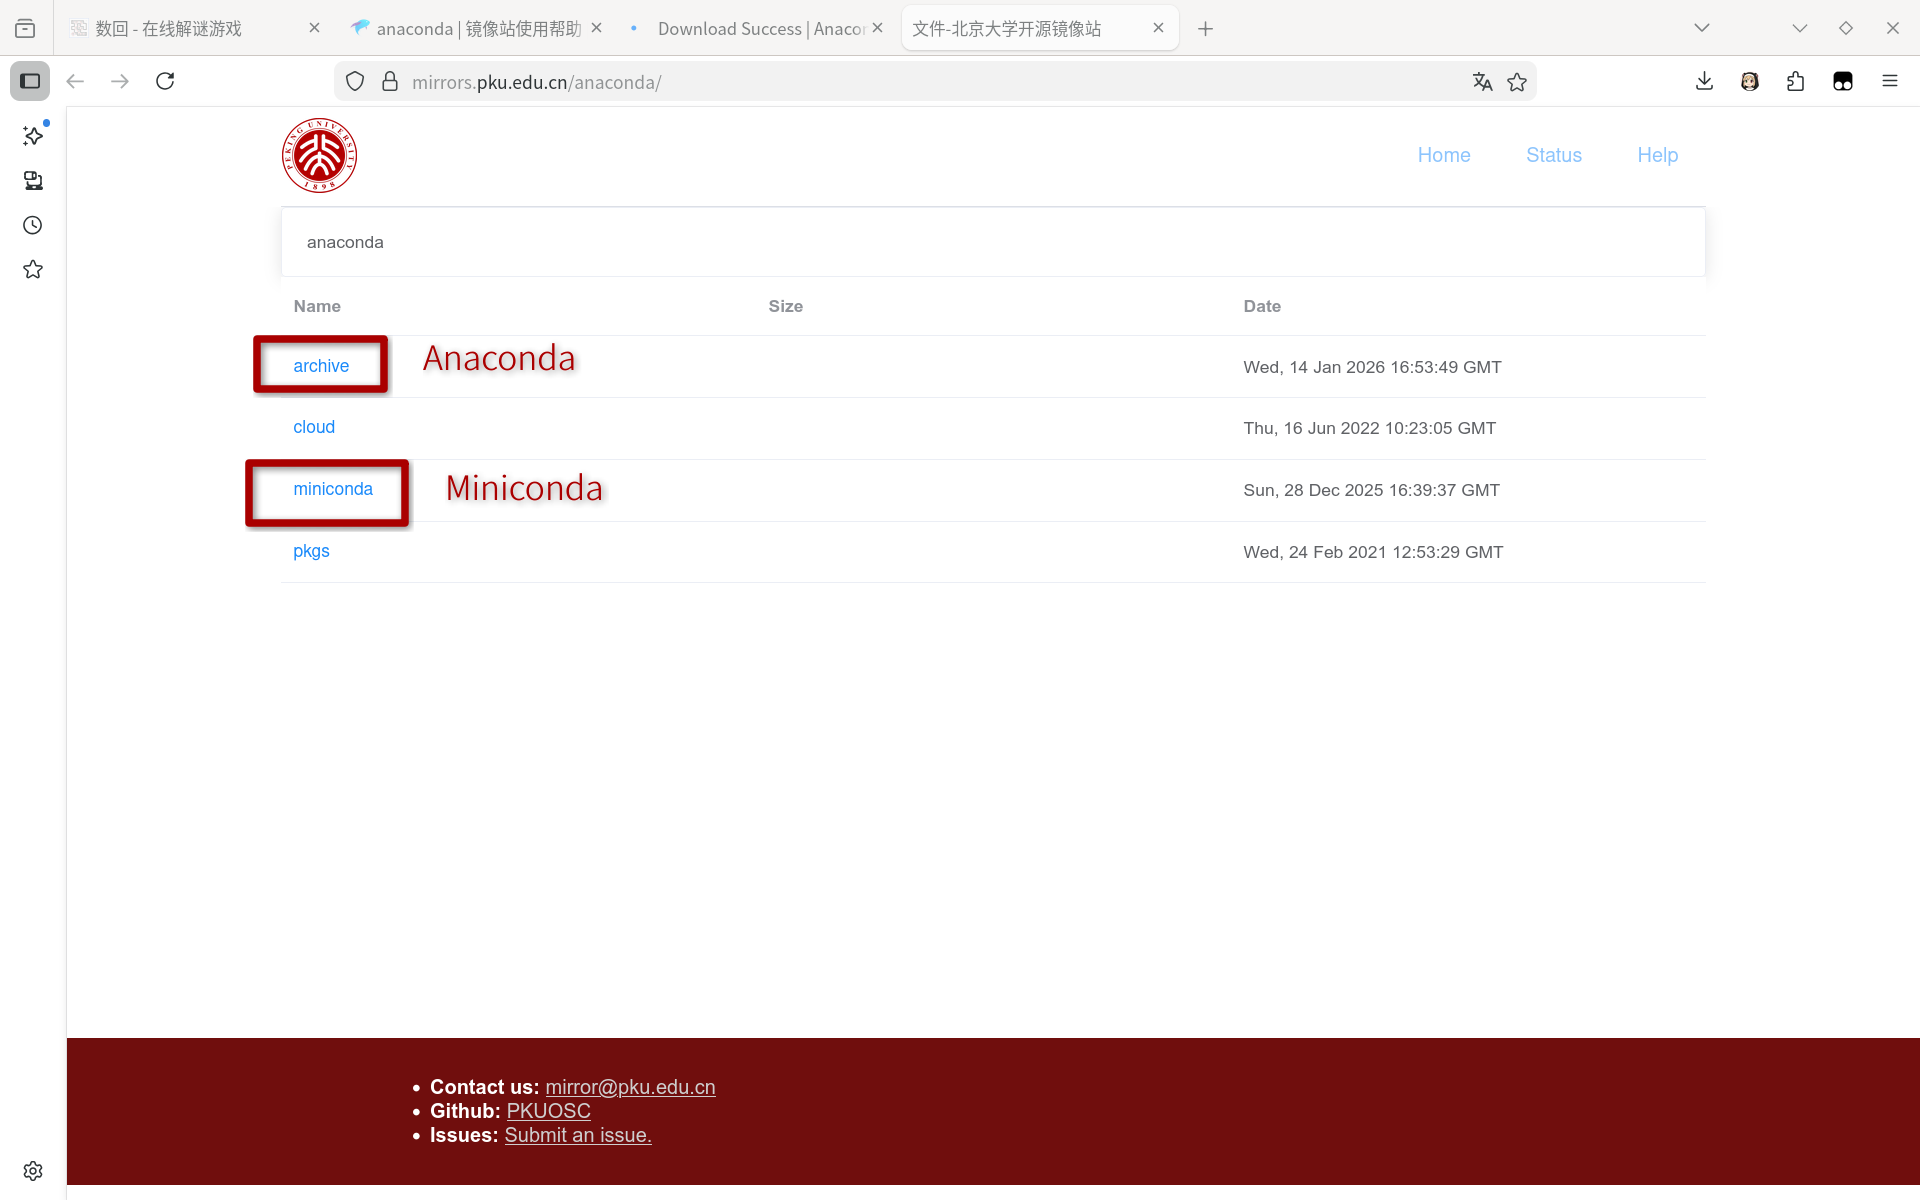
\includegraphics[width=0.8\textwidth]{pku-mirror.png}
\end{figure}

选择适合你操作系统的最新版本（Windows、macOS、Linux），点击下载。

\paragraph{清华源} 访问\url{https://mirrors.tuna.tsinghua.edu.cn/anaconda/}。

\begin{figure}[htbp]
    \centering
    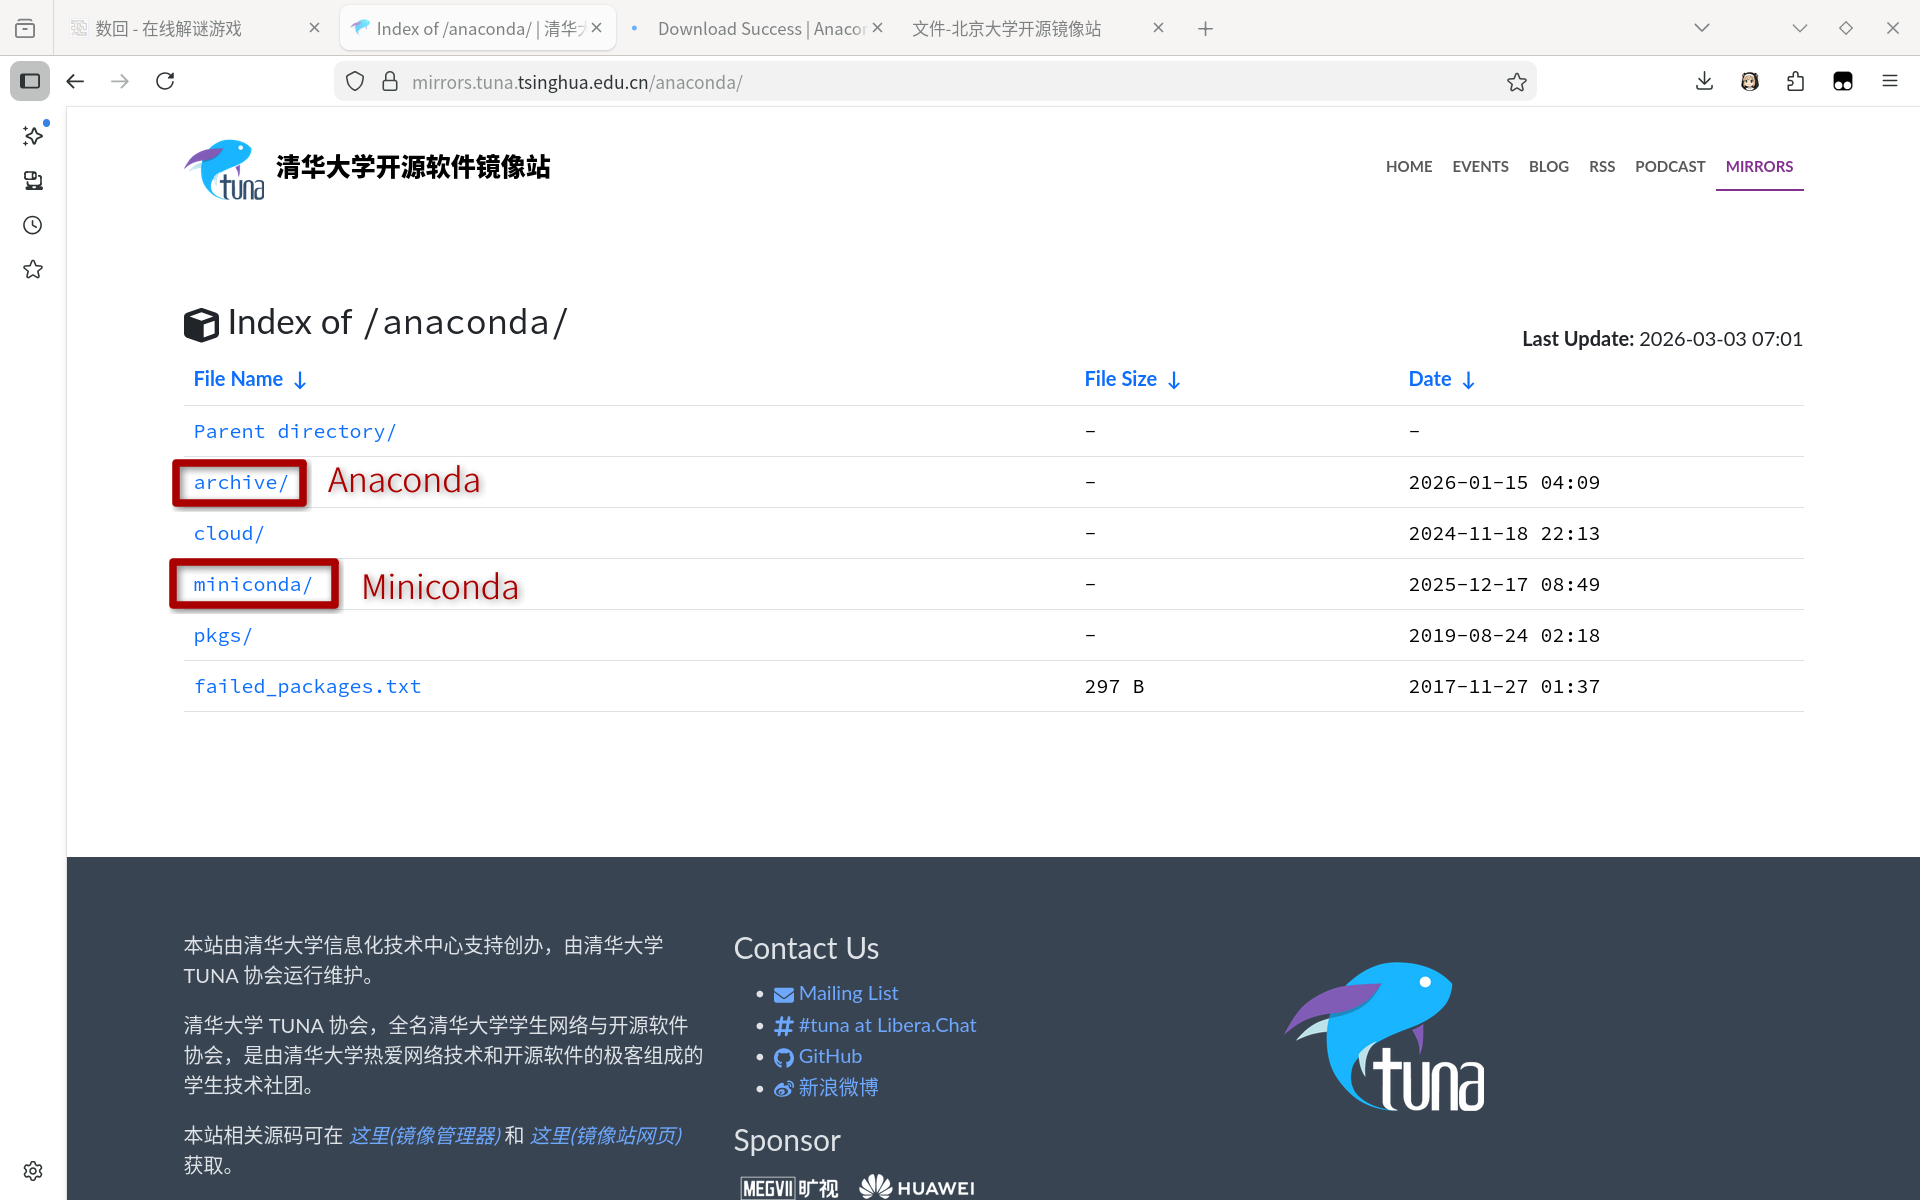
\includegraphics[width=0.8\textwidth]{thu-mirror.png}
\end{figure}

同样选择适合你操作系统的最新版本，点击下载。

\section{安装Anaconda}

刚刚下载的是一个安装包。我们应当运行该安装包进行安装。安装过程非常简单，基本上按照提示点击“下一步”即可。安装过程中会有一些选项，其中有一项“Add Anaconda to my PATH environment variable”，新手建议勾选它，这样在命令行中就可以直接使用conda命令了\footnote{仅在Windows中，该选项会导致一些问题。但是你既然已经是新手了，那这个问题对你而言是非常遥远的，完全不必在意，也不要在意部分LLM或教程要求的“绝对不要勾选”，尽管勾选即可。确信自己不是新手的，可以自行查找“conda cli”相关的教程。}。

安装之后，重启你的计算机。

重启之后，随便开一个终端\footnote{按\texttt{Win + R}，输入\texttt{cmd}或\texttt{powershell}，回车打开一个新的终端窗口。如果你是Linux，按\texttt{Ctrl + Alt + T}打开一个新的终端窗口。如果你是macOS，按\texttt{Command + Space}，输入\texttt{Terminal}，回车打开一个新的终端窗口。
}，键入以下命令并回车执行：
\begin{minted}{bash}
conda --version
\end{minted}
如果终端输出了conda的版本号，说明安装成功了。

然后运行一下
\begin{minted}{bash}
conda init --all
\end{minted}
该命令会为你的终端配置conda的环境变量，使得你在任何终端中都可以使用conda命令。

如果终端提示“conda: command not found”或者类似的错误，说明安装过程中可能出现了问题，八成是没有将conda添加到环境变量中。\textbf{只要你在刚才听从了我的建议，勾选了“Add Anaconda to my PATH environment variable”，就不应该出现这个问题。}如果你没有勾选那个选项，那么你需要自行查找相关资料解决这个问题了，毕竟你已经自认为不是新手了。

\section{换源}

\subsection{为conda换源}

conda默认使用官方源进行包管理，这个源在国内访问速度非常慢，所以我们需要换源。

换源并不需要重新安装什么可执行文件！

以清华源为例，我们访问\url{https://mirrors.tuna.tsinghua.edu.cn/}，映入眼帘的应该是这个界面：

\begin{figure}[htbp]
    \centering
    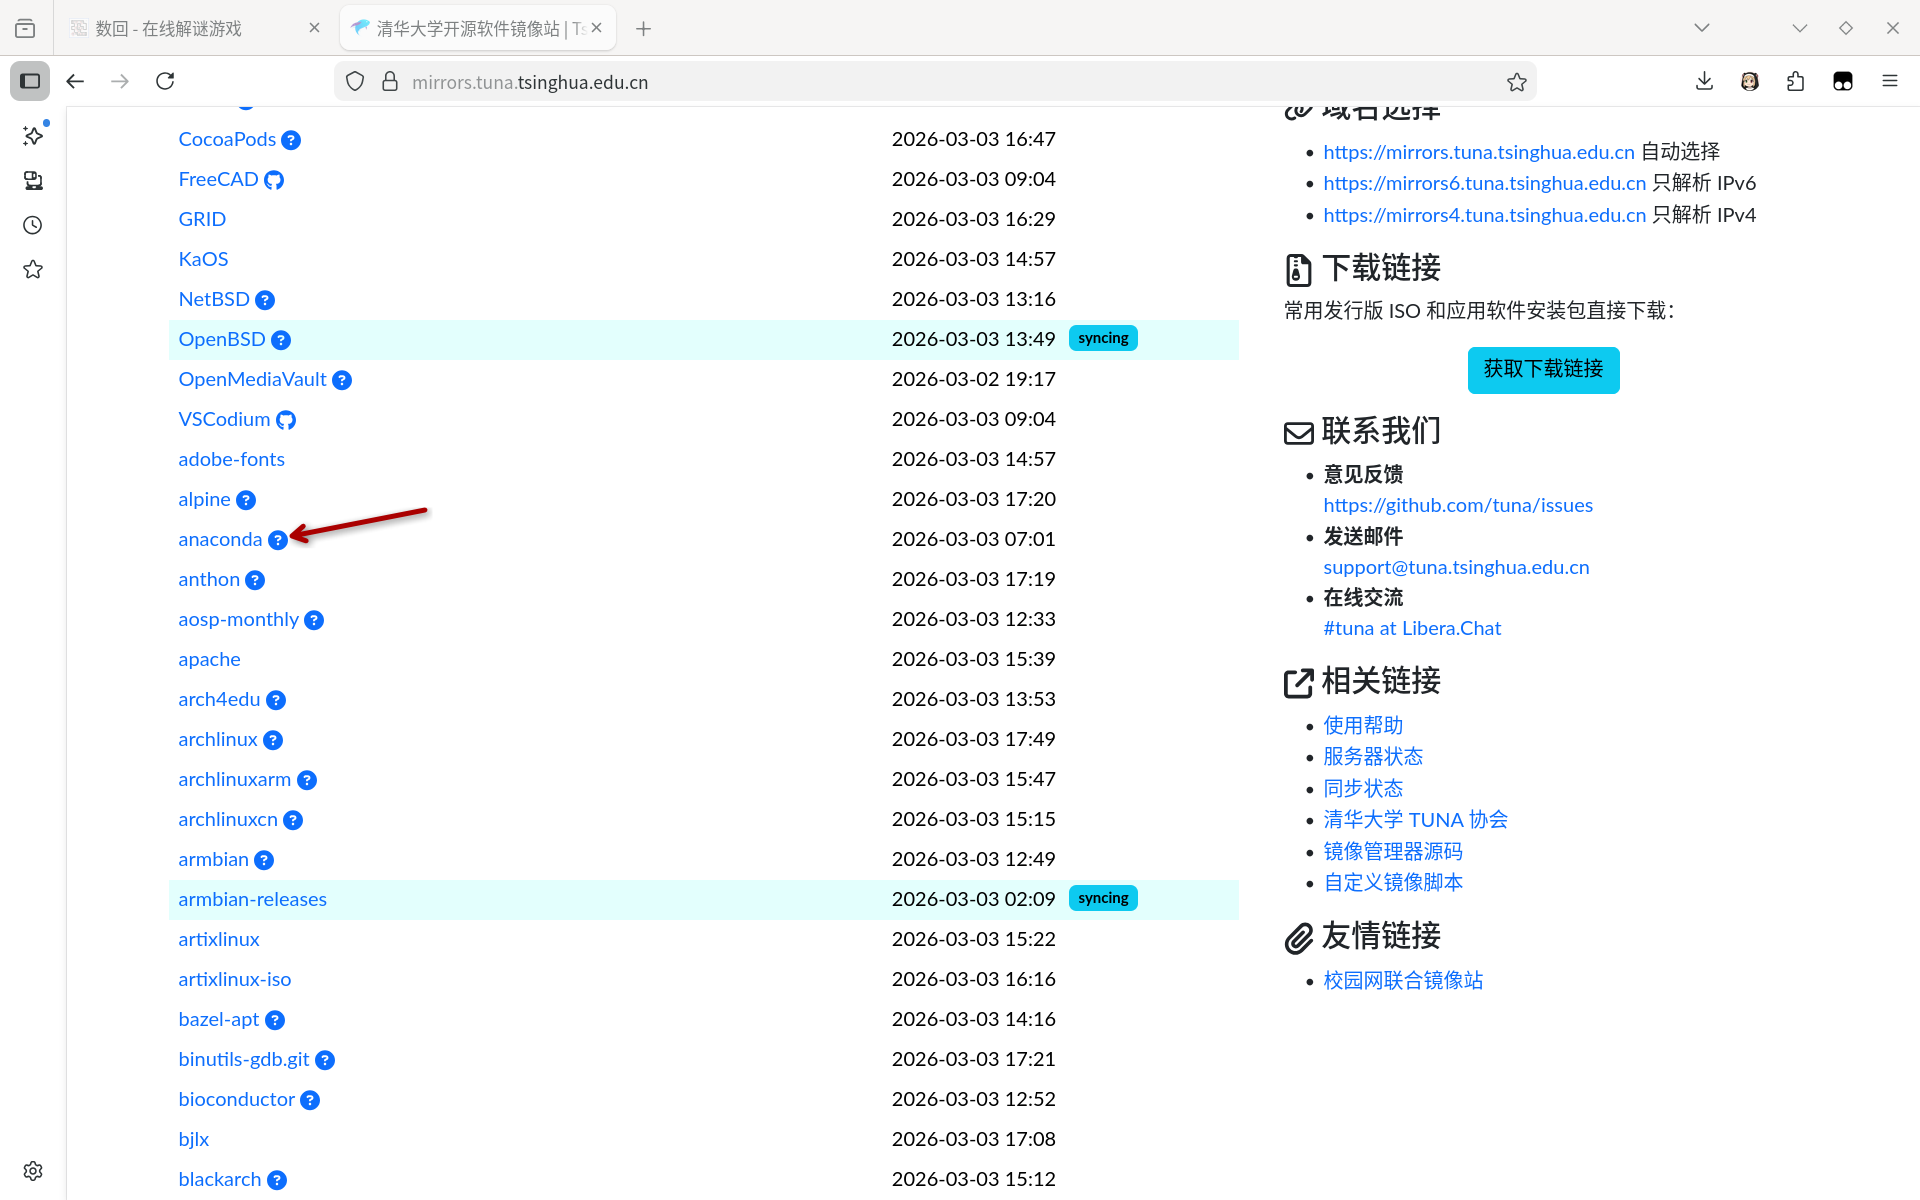
\includegraphics[width=0.8\textwidth]{thu-change.png}
\end{figure}
看到anaconda这行字右边的“使用说明”了吗？点击它，里面有详细的换源教程。按照教程操作即可。

对于看不懂教程的人，我也可以在这里翻译一遍。

\begin{enumerate}
    \item 打开终端，输入以下命令并回车执行：
    \begin{minted}{bash}
conda config --set show_channel_urls yes
    \end{minted}
    \item 找到一个叫做 \texttt{.condarc} 的文件。这个文件通常在你的用户目录下（Windows上是\texttt{C:\textbackslash Users\textbackslash 你的用户名}，Linux和macOS上是\texttt{/home/你的用户名}）。\textbf{如果你刚刚运行了上面的命令，那么这个文件应该已经被创建了。}
    \item 用文本编辑器（比如Windows上的记事本，Linux和macOS上的vim或nano）打开这个\texttt{.condarc}文件。
    \item 在文件中，用以下内容替换掉原有的内容（如果原有内容不为空的话）。注意缩进和格式必须保持一致。
    \begin{minted}{yaml}
channels:
  - defaults
show_channel_urls: true
default_channels:
  - https://mirrors.tuna.tsinghua.edu.cn/anaconda/pkgs/main
  - https://mirrors.tuna.tsinghua.edu.cn/anaconda/pkgs/r
  - https://mirrors.tuna.tsinghua.edu.cn/anaconda/pkgs/msys2
custom_channels:
  conda-forge: https://mirrors.tuna.tsinghua.edu.cn/anaconda/cloud
  pytorch: https://mirrors.tuna.tsinghua.edu.cn/anaconda/
    \end{minted}
    \item 保存并关闭文件。
\end{enumerate}

北大源的换源教程和它类似。

\subsection{为pip换源}

只要你看了我的上一个讲义，你就会知道pip也是需要换源的。pip默认使用官方源进行包管理，这个源在国内访问情况比conda要好些，不过还是建议换源。

当然前提是你的虚拟环境里已经装了python和pip。运行以下命令安装python和pip：
\begin{minted}{bash}
conda install python pip
\end{minted}

同样的，以清华源为例。

\begin{enumerate}
    \item 打开终端，输入以下命令并回车执行：
    \begin{minted}{bash}
python -m pip install --upgrade pip
    \end{minted}
    该命令会升级pip到最新版本，确保我们有最新的功能和修复。
    \item 再运行以下命令：
    \begin{minted}{bash}
pip config set global.index-url https://mirrors.tuna.tsinghua.edu.cn/pypi/web/simple
    \end{minted}
    该命令会将pip的默认源设置为清华源。
    \item 关闭终端并重新打开，以确保配置生效。
\end{enumerate}

\end{document}